\documentclass[a4paper,11pt]{report}

\usepackage{amsmath}
\usepackage{fullpage}
\usepackage{bussproofs}
\usepackage{mathpartir}
\usepackage{prooftrees}
\usepackage{color}

\usepackage{tikz}
\usetikzlibrary{automata,positioning}

\author{Sylvain Julmy}
\date{\today}

\setlength{\parindent}{0pt}

\newcommand*{\equal}{=}

\begin{document}

\begin{center}
  \large{
    Formal Methods\\
    Fall 2017
  }
  
  \noindent\makebox[\linewidth]{\rule{\linewidth}{0.4pt}}
  S03
  \noindent\makebox[\linewidth]{\rule{\linewidth}{0.4pt}}

  \begin{flushleft}
    Professor : Ultes-Nitsche Ulrich

    Assistant : Christophe Stammet
  \end{flushleft}

  
  \noindent\makebox[\linewidth]{\rule{\linewidth}{0.4pt}}

  Submitted by Sylvain Julmy
  
  \noindent\makebox[\linewidth]{\rule{\textwidth}{1pt}}
\end{center}

\section*{Exercise 1}

\begin{align*}
  F \equiv & (C \vee \neg A) \wedge D \wedge (D \vee A) \wedge (E \vee B) \wedge \\
           & (\neg C \vee A \vee B) \wedge E \wedge (\neg D \vee \neg A) \wedge \\
           & (C \vee \neg B) \wedge (\neg E \vee \neg B) \wedge C
\end{align*}

\subsection*{Applying the resolution}

\subsubsection*{Using $A$}

\begin{gather*}
  (C \vee \neg A) \wedge (D \vee A) \wedge (\neg C \vee A \vee B) \wedge (\neg D
  \vee \neg A) \wedge \cdots = \\
  (C \vee D) \wedge \underbrace{(\neg D \vee D)}_\top \wedge
  \underbrace{(C \vee \neg C \vee B)}_\top \wedge (\neg C \vee \neg D \vee B)
  \wedge \cdots = \\
  (C \vee D) \wedge (\neg C \vee \neg D \vee B) \wedge (E \vee B) \wedge (C \vee
  \neg B) \wedge (\neg E \vee \neg B) \wedge D \wedge E \wedge C
\end{gather*}

\subsubsection*{Using $C$}

\begin{gather*}
  (C \vee D) \wedge (\neg C \vee \neg D \vee B) \wedge (C \vee \neg B)
  \wedge C \wedge \cdots = \\
  \underbrace{(D \vee \neg D \vee B)}_\top \wedge \underbrace{(\neg B \vee B
    \vee \neg D)}_\top \wedge (\neg D \vee B) \wedge D \wedge E \wedge (E \vee
  B) \wedge (\neg E \vee \neg B) = \\
  (\neg D \vee B) \wedge D \wedge E \wedge (E \vee B) \wedge (\neg E \vee \neg B)
\end{gather*}

\subsubsection*{Using $E$}

\begin{gather*}
  (\neg D \vee B) \wedge D \wedge E \wedge (E \vee B) \wedge (\neg E \vee \neg
  B) = \\
  \underbrace{(B \vee \neg B)}_\top \wedge \neg B \wedge D \wedge (\neg D \vee
  B) = \\
  \neg B \wedge D \wedge (\neg D \vee B)
\end{gather*}

\subsubsection*{Using $B$}

\begin{gather*}
  \neg B \wedge D \wedge (\neg D \vee B) = \\
  D \wedge \neg D = \bot
\end{gather*}

because $F \equiv \bot$, the formula is not satisfiable.

\section*{Exercice 2}

We suppose that we have a function $tester(P)$ which test if the program $P$
will stop or not :
\begin{itemize}
\item If $P$ stops, tester return $true$
\item Else, it return $false$.
\end{itemize}

Now, we create the following program :
\begin{verbatim}
tester2(P) = 
  if (tester(P)
    then loop forever
    else true
\end{verbatim}

Now we call $tester2$ with $tester2$ : \verb|tester2(tester2)|. And we have the
contradiction : $tester2$ loop forever if and only if $tester$ accept $tester2$
and if and only if $tester2$ end, which is impossible because $tester$ has to
accept $tester2$. So it is a proof that the program $tester$ can't exist.

\section*{Exercice 3}

\subsection*{Formal description of $M_1$}

\[
  M_1 : (\{q_0,q_1,q_2,q_3\},\{0,1\},\{0,1,B\},\delta,q_0,B,\{q_3\})
\]

where

\begin{align*}
  \delta(q_0,0) &= (q_1,B,R) \\
  \delta(q_0,1) &= (q_2,B,R) \\
  \delta(q_1,0) &= (q_1,0,R) \\
  \delta(q_1,1) &= (q_2,0,R) \\
  \delta(q_1,B) &= (q_3,0,R) \\
  \delta(q_2,B) &= (q_3,1,R) \\
  \delta(q_2,1) &= (q_2,1,R) \\
  \delta(q_2,0) &= (q_1,1,R)
\end{align*}

This Turing machine implements a right shift on binary number, it multiply a
binary number by $2$ (or divide it by $2$, depending on which direction we represent
the number...)

\subsection*{Finite state represantation of $M_2$}

\begin{center}
  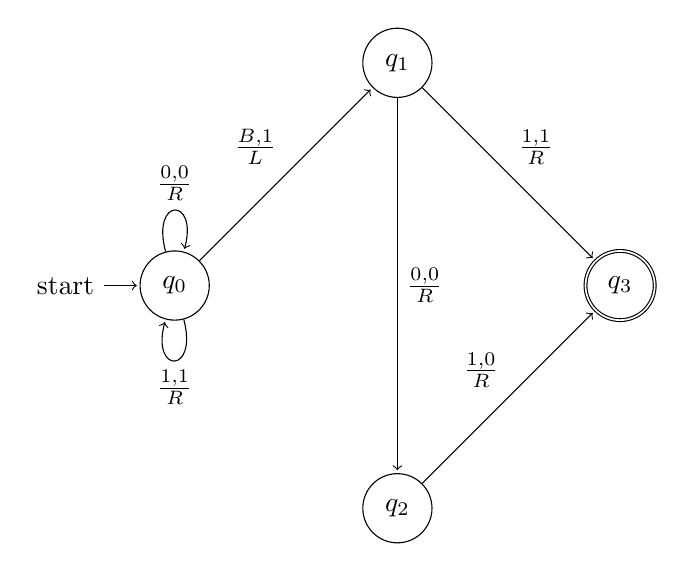
\begin{tikzpicture}[shorten >=1pt,node distance=4cm,on grid,auto]
    \node[state,initial] (q_0) [] {$q_0$};
    \node[state] (q_1) [above right of = q_0]{$q_1$};
    \node[state] (q_2) [below right of = q_0]{$q_2$};
    \node[state,accepting] (q_3) [below right of = q_1] {$q_3$};
    \path[->]
    (q_0) edge [loop above] node {$\frac{0,0}{R}$} ()
          edge [loop below] node {$\frac{1,1}{R}$} ()
          edge node {$\frac{B,1}{L}$} (q_1)
    (q_1) edge [] node {$\frac{0,0}{R}$} (q_2)
          edge [] node {$\frac{1,1}{R}$} (q_3)
    (q_2) edge node {$\frac{1,0}{R}$} (q_3)
          ;
  \end{tikzpicture}
\end{center}

This Turing machine add the last (right most) digit of a number to his end , for example
$0101$ give $01011$ and $0100$ give $01000$.

\end{document}

%%% Local Variables:
%%% mode: latex
%%% End:
